\begin{center}
\begin{LARGE}
\title{\textbf{Labirynty}}
\author{Zuzanna Pawłowska}
\end{LARGE}
\end{center}

\maketitle
\section{Historia labiryntów}
\subsection{Mityckie korzenie}
\begin{flushleft}
Historia labiryntów ma korzenie sięgające starożytności. Jednym z najbardziej znanych labiryntów był ten z \textit{Krety}, stworzony według mitologii greckiej przez \textbf{Dédala}, aby uwięzić \textbf{Minotaura}. Labirynt ten był tak skomplikowany, że trudno było znaleźć drogę wyjścia.
\end{flushleft}

\subsection{Istotna symbolika}
\begin{center}
Labirynty były również popularnymi elementami w \underline{starożytnych egipskich grobowcach} i katedrach chrześcijańskich, symbolizując duchową wędrówkę lub inicjację. W średniowieczu, malarze często przedstawiali labirynty jako metafory życiowych wyzwań i prób.
\end{center}

\subsection{Aktualnie}
\begin{flushright}
Obecnie labirynty często służą celom rekreacyjnym i medytacyjnym. Współczesne labirynty, takie jak słynny Labirynt Chartres, przyciągają ludzi pragnących znaleźć spokój i kontemplację w ich zakręconych ścieżkach.\par Historia labiryntów jest fascynującym przykładem, jak ten symboliczny wzór ewoluował i zmieniał się przez wieki.(Przykładowy labirynt \ref{fig:labirynt} znajduje się na \pageref{fig:labirynt} stronie.
\end{flushright}

\subsection{Rodzaje labiryntów}
\begin{itemize}
    \item Jednokierunkowe labirynty: Osoba wchodzi i podąża przez jeden, zaplanowany kierunek.
    \item Dwukierunkowe labirynty: Osoba może wybierać różne ścieżki, aby dotrzeć do celu.
    \item Labirynty logiczne: Zadania lub łamigłówki, które polegają na rozwiązaniu problemu, aby przejść przez labirynt.
    \item Labirynty wirtualne: Tworzone za pomocą oprogramowania komputerowego lub gier wideo.
    \item Labirynty na świeżym powietrzu: Często występują w parkach i ogrodach jako atrakcje dla zwiedzających. 
\end{itemize}

\subsection{Przykładowy labirynt}
\begin{figure}[hbt!]
    \centering
    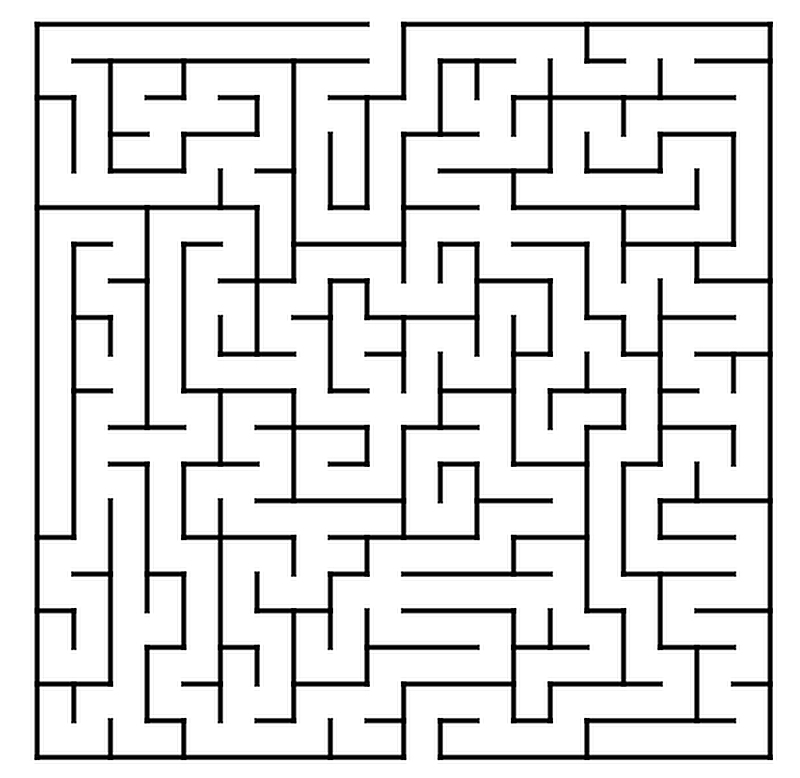
\includegraphics{pictures/labirynt.jpg}
    \caption{Przykład labiryntu}
    \label{fig:labirynt}
\end{figure}


\subsection{Zalecenia dotyczące nawigacji w labiryntach}
\begin{enumerate}
    \item Zachowaj spokój i koncentrację.
    \item Staraj się zaplanować trasę i przewiduj przyszłe ruchy.
    \item Często obserwuj otoczenie, aby uniknąć błędów.
\end{enumerate}

\subsection{Równanie rekurencyjne do obliczania liczby możliwych ścieżek w labiryncie o rozmiarze n x m, zakładając, że można poruszać się tylko w górę i w prawo:}
\[R(n, m) = R(n-1, m) + R(n, m-1)\]

\subsection{Zmiany dodane za pomocą Overleafa}

\subsection{Podsumowanie}
\begin{table}[hbt!]
\begin{tabular}{|l|l|l|l|l|}
\hline
\textbf{Numer} & \textbf{Labirynt}      & \textbf{Trudność} & \textbf{Rodzaj} & \textbf{Zastosowanie} \\ \hline
\textbf{1.}    & Labirynt Knossos       & Średnia           & Historyczny     & Edukacja              \\ \hline
\textbf{2.}    & Labirynt Hampton Court & Trudna            & Historyczny     & Rozrywka              \\ \hline
\textbf{3.}    & Labirynt w parku       & Łatwa             & Ogrodowy        & Rekreacja             \\ \hline
\textbf{4.}    & Labirynt w grze wideo  & Różna             & Wirtualny       & Rozrywka              \\ \hline
\end{tabular}
\end{table}
